You can automatically report the status of an automated test to an external system. The reporting is achieved by writing a comment on a task in the external repository. The comment includes a link to the test result in the dasboard. 

\subsubsection{Configuring a task repository for your \gdproject{}}
\label{TasksALMConfigureProject}
Once you have configured one or more repositories for your workspace \bxpref{TasksALMConfigureWorkspace}, you can select one of these to be the test-relevant repository for your \gdproject{}. 

This will let you:
\begin{itemize}
\item Add a task ID from this repository to \gdcases{} and \gdsuites{} in the \gdproject{} to signify that this item is the test for this task \bxpref{TasksALMAddTask}.
\item Automatically report test results to the task defined when a test runs.
\item View the test results for the relevant item in the dashboard as a link from the task repository.
\end{itemize}

\textbf{To configure a task repository for your \gdproject{}:}

\begin{enumerate}
\item In the \gdproject{} Properties, select \bxname{Mylyn ALM} from the tree on the left \bxfigref{TasksALMProjectProperties}.
\item In the page that appears, you can select a repository from the combo-box. You can validate the repository settings using the button.
\item You can then choose whether to only report failed tests, only report successful tests, or both.
\item Enter the URL of the \dash{} that is configured to use the correct \gddb{} for your test results. This is the \dash{} that will be opened when you click on a test result link from the task repository. For more information on configuring and starting the \dash{}, see the documentation \bxpref{TasksDashboard}.
\end{enumerate}

\begin{figure}[h]
\begin{center}
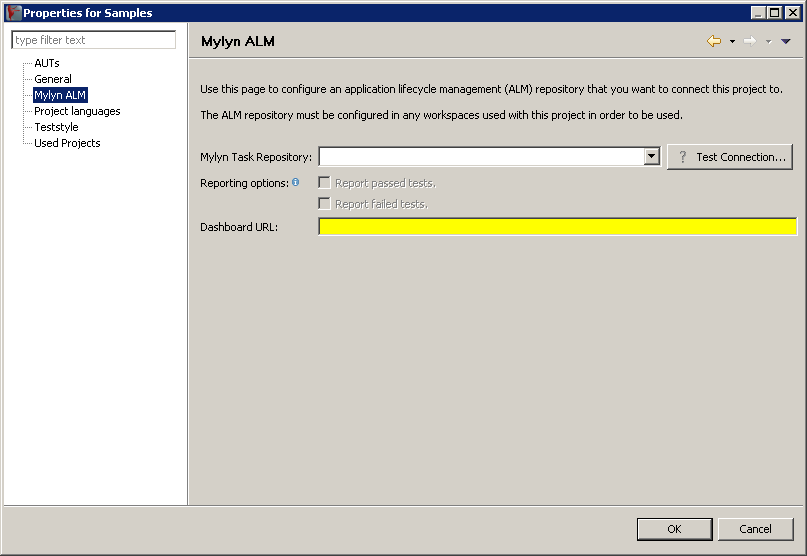
\includegraphics[width=12.5cm]{Tasks/ALM/PS/almproperties}
\caption{ALM Settings}
\label{TasksALMProjectProperties}
\end{center}
\end{figure}



\subsubsection{Adding task IDs to \gdjobs{}, \gdsuites{} and \gdcases{}}
\label{TasksALMAddTask}

You can add a task ID to \gdcases{} and \gdsuites{} in your \gdproject{}. 

The task ID should be a valid ID in the repository that you have specified as the repository for this \gdproject{} \bxpref{TasksALMConfigureProject}. Adding the task ID to an item in your \gdproject{} means that this item is the relevant test for that task in your repository. You will be able to report test results for this item as a comment to the task in the repository. The comment will include a link to the dashboard, in which the test result report can be viewed.

To add a task ID to a \gdcase{} or \gdsuite{}:
\begin{enumerate}
\item Open the item in the editor by double-clicking it.
\item In the \gdpropview{}, in the cell for \bxname{Task ID}, enter the task ID from the external repository. You can only enter task IDs at the place of specification -- you cannot overwrite them when you reuse the item.
\item Save the editor. 
\item When you have added a task ID to a node, you can open the task for this node from the browser by selecting:\\
\bxmenu{Open with}{Mylyn Task Editor}{}
\end{enumerate}

\bxtipp{You should ensure that you add task IDs to the right node-level to provide you with the relevant amount of information for the tasks in your repository. This will usually be at the level of Use Cases within a \gdsuite{}. }

\subsubsection{Test execution with reporting to external repositories}
If your \gdproject{} is joined to an external repository \bxpref{TasksALMConfigureProject}, and you have added task IDs to one or more items in your \gdproject{} \bxpref{TasksALMAddTask}, then the following will happen after a test has run:

\begin{itemize}
\item The test results are analyzed to see if any comments need to be added inthe external repository (you can deactivate commenting for failed nodes or successful nodes in the \gdproject{} properties). 
\item If there are comments to be added, \ite{} connects to the repository and writes one comment per task, as defined in the \gdproject{} properties. If multiple items reference the same task ID, or if an item with a task ID is executed multiple times,  then each test status and result link is written, but all in one comment. 
\bxtipp{Tests that have a status other than \bxname{passed} (e.g. failed, stopped, still testing) are considered as \bxname{failed}.}
\item You can see the status of the ALM reporting in the console view. 
\item Once a comment has been written, you can see the comment in the external repository. From there, you can click on the link provided to open the test result report in the \dash{} that you specified for your \gdproject{}. The \dash{} must be already running for this action to succeed. The test results must also still be present in the \gddb{} \bxpref{TasksReopenTestResult}.
\item In the test result report, the test result report is opened at the node which referenced the current task ID. 
\end{itemize}

\bxwarn{This option is currently only supported for tests started via the \ite{}}
